\documentclass[tikz,border=6pt]{standalone}
\usepackage{amsmath}
\usetikzlibrary{arrows.meta,positioning,calc}
\begin{document}
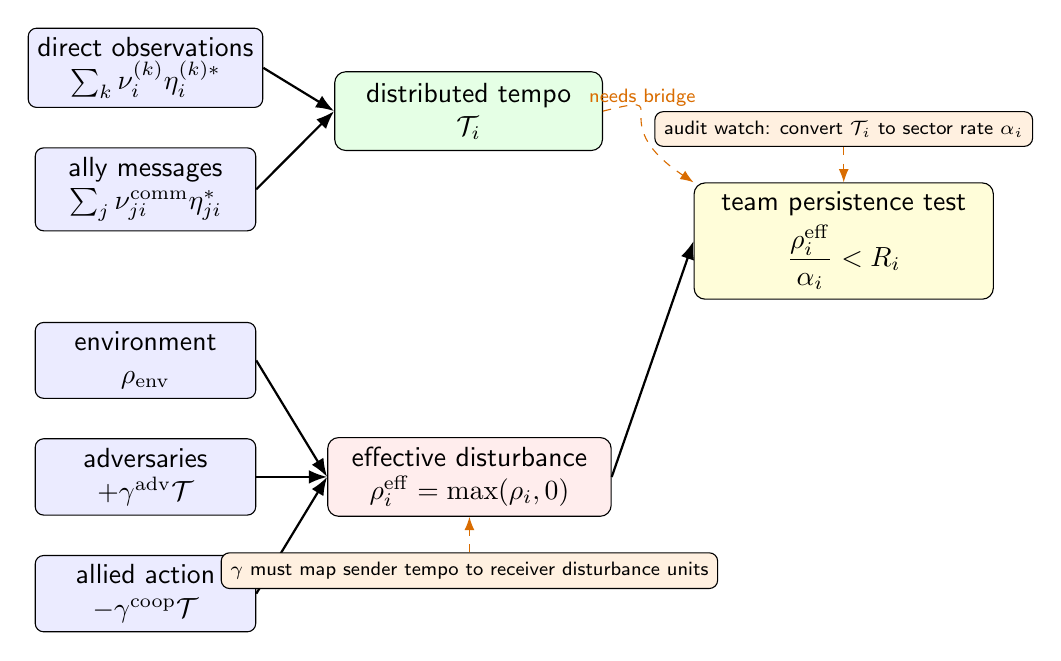
\begin{tikzpicture}[
  font=\sffamily,
  >=Latex,
  source/.style={draw, rounded corners=3pt, fill=blue!8, align=center, minimum width=2.8cm, minimum height=0.72cm},
  box/.style={draw, rounded corners=4pt, fill=green!10, align=center, minimum width=3.4cm, minimum height=1.0cm},
  rho/.style={draw, rounded corners=4pt, fill=red!7, align=center, minimum width=3.6cm, minimum height=1.0cm},
  test/.style={draw, rounded corners=4pt, fill=yellow!15, align=center, minimum width=3.8cm, minimum height=1.05cm},
  warn/.style={draw, rounded corners=3pt, fill=orange!12, align=center, font=\sffamily\scriptsize}
]

\node[source] (obs) {direct observations\\$\sum_k \nu_i^{(k)}\eta_i^{(k)*}$};
\node[source, below=0.5cm of obs] (comm) {ally messages\\$\sum_j \nu_{ji}^{\rm comm}\eta_{ji}^*$};
\node[box, right=0.9cm of obs, yshift=-0.55cm] (tempo) {distributed tempo\\$\mathcal T_i$};

\draw[->, thick] (obs.east) -- (tempo.west);
\draw[->, thick] (comm.east) -- (tempo.west);

\node[source, below=1.15cm of comm] (env) {environment\\$\rho_{\rm env}$};
\node[source, below=0.5cm of env] (adv) {adversaries\\$+\gamma^{\rm adv}\mathcal T$};
\node[source, below=0.5cm of adv] (coop) {allied action\\$-\gamma^{\rm coop}\mathcal T$};
\node[rho, right=0.9cm of adv] (effrho) {effective disturbance\\$\rho_i^{\rm eff}=\max(\rho_i,0)$};

\draw[->, thick] (env.east) -- (effrho.west);
\draw[->, thick] (adv.east) -- (effrho.west);
\draw[->, thick] (coop.east) -- (effrho.west);

\node[test, right=1.15cm of tempo, yshift=-1.65cm] (persist)
  {team persistence test\\[2pt]$\displaystyle \frac{\rho_i^{\rm eff}}{\alpha_i}<R_i$};

\draw[->, thick] (effrho.east) -- (persist.west);
\draw[->, dashed, orange!85!black] (tempo.east) .. controls +(1.0,0.25) and +(-1.2,0.8) .. node[above, font=\sffamily\scriptsize] {needs bridge} (persist.north west);

\node[warn, above=0.45cm of persist, minimum width=4.2cm] (bridge)
  {audit watch: convert $\mathcal T_i$ to sector rate $\alpha_i$};
\draw[->, dashed, orange!85!black] (bridge.south) -- (persist.north);

\node[warn, below=0.45cm of effrho, minimum width=4.3cm] (units)
  {$\gamma$ must map sender tempo to receiver disturbance units};
\draw[->, dashed, orange!85!black] (units.north) -- (effrho.south);

\end{tikzpicture}
\end{document}
